%%%% Paramétrage du TD %%%%
\def\xxactivite{Révisions \ifprof -- Corrigé \else \fi} % \normalsize \vspace{-.4cm}
\def\xxauteur{\textsl{Xavier Pessoles}}


\def\xxnumchapitre{Révisio  \vspace{.2cm}}
\def\xxchapitre{\hspace{.12cm} Résolution des problèmes de cinématique -- Cinématique du contact ponctuel}
\def\xxonglet{\textsf{Rév -- Cin}}
\def\xxactivite{TD 01}
\def\xxauteur{\textsl{Renan Bonnard}}

\def\xxpied{%
Révision cinématique -- Résolution des problèmes de cinématique\\
Fiche 1 -- \xxactivite%
}

\def\xxcompetences{%
\textsl{%
\textbf{Savoirs et compétences :}\\
%\vspace{-.4cm}
%\begin{itemize}[label=\ding{112},font=\color{ocre}] 
%%\item \textit{Res1.C4 : } Correction
% \item \textit{Res1.C4.SF1 : } Proposer la démarche de réglage d’un correcteur proportionnel
%%proportionnel intégral 
%%et à avance de phase
%\item \textit{Con.C2 : } 	Correction d’un système asservi	
%\item \textit{Con.C2.SF1 : } Choisir un type de correcteur adapté
%\end{itemize}
}}

\def\xxauteur{\textsl{Renan Bonnard}}

\def\xxtitreexo{Guidage linéaire de systèmes médicaux}
\def\xxsourceexo{\hspace{.2cm} \footnotesize{}}

\def\xxfigures{
%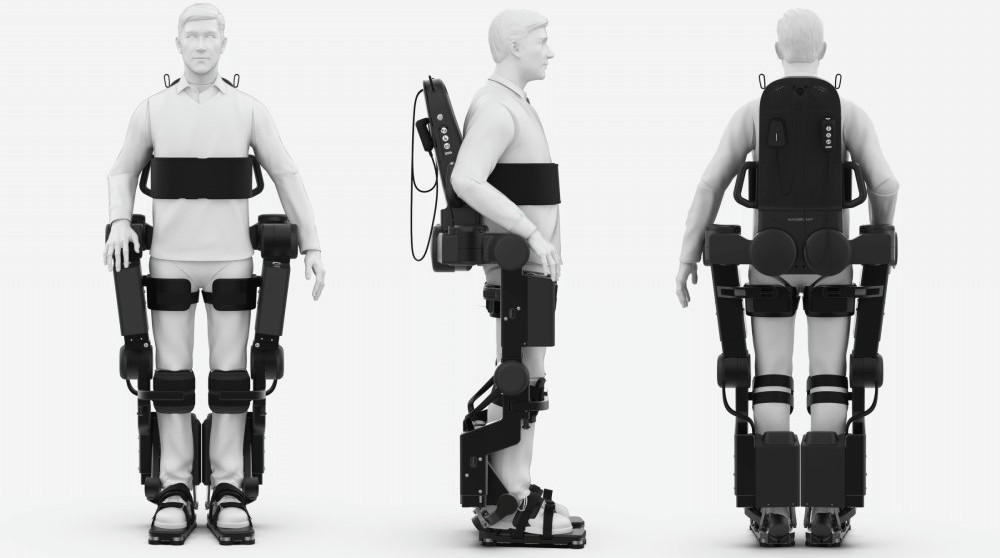
\includegraphics[width=.55\textwidth]{fig_00}
}%figues de la page de garde

\input{\repStyle/pagegarde_TD.tex}
\vspace{4cm}


\ifprof
\else
\begin{multicols}{2}
\fi





L’étude suivante porte sur le guidage en translation d’un chariot 
de scanner médical S1 par rapport au bâti de la machine S0. Ce 
guidage est réalisé par deux séries de billes, S2 et S3, qui roulent 
dans des rainures en V. 
\begin{center}
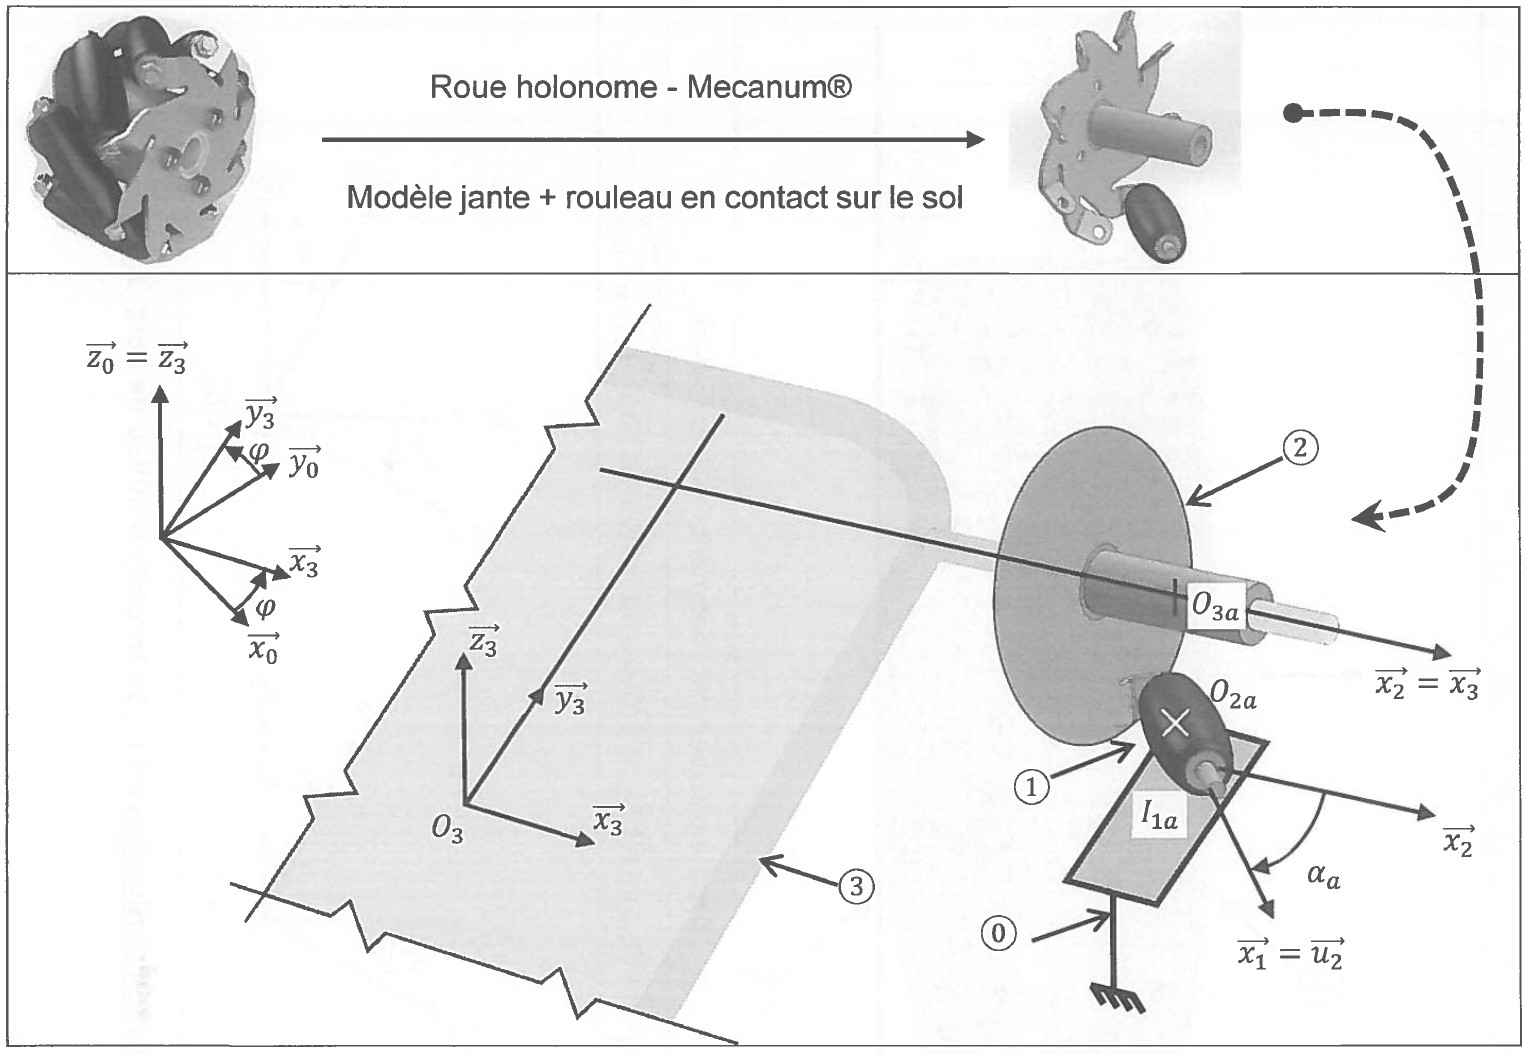
\includegraphics[width=.95\linewidth]{fig_04}
\end{center}

La figure ci-dessous présente, en coupe, la réalisation technologique de ce guidage. 

\begin{center}
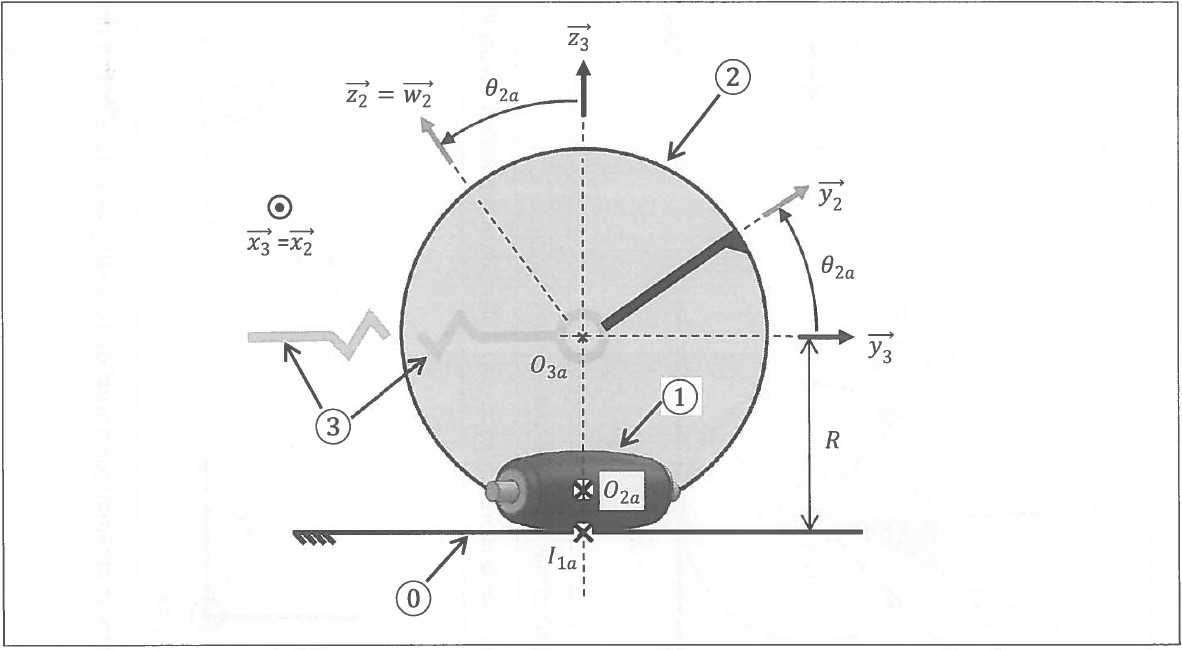
\includegraphics[width=\linewidth]{fig_05}
\end{center}

Les billes S2 de rayon $R$ roulent sans glisser sur les plans d’une rainure en V d’angle égal à 90\textdegree usinée dans 
S1 et sur les plans d’une autre rainure en V d’angle égal à 120\textdegree usinée dans S0. 
Les billes S3 de rayon $r$ roulent sans glisser sur les plans d’une rainure en V d’angle égal à 
$2\alpha$ usinée dans 
S1 et sur le plan (P) de S0. 

On note $\torseurcin{V}{1}{0}=\torseurl{\vect{0}}{v\vect{x}}{\forall P}$ le torseur cinématique du mouvement du chariot S1 par rapport au bâti S0. 

On pose $\vecto{2}{0} = \omega_{20}\vect{y}$ et $\vecto{3}{0} = \omega_{30}\vect{y}$.

\question{Traduire les conditions de non glissement. En déduire quelques axes instantanés de rotation.}
\ifprof
\begin{corrige}
\end{corrige} \else \fi

\question{Déterminer $\vectv{C}{2}{0}$ en fonction de $v$, puis $\vectv{E}{3}{0}$ en fonction de $v$. Déterminer $\vectv{C}{2}{0}$ en fonction de $\omega_{20}$, puis $\vectv{E}{3}{0}$ en fonction de $\omega_{30}$. En déduire une relation entre $\omega_{20}$ et $v$, puis une relation entre $\omega_{30}$ et $v$.}
\ifprof
\begin{corrige}
\end{corrige} \else \fi

\question{En déduire les torseurs cinématiques des mouvements de S2/S0 et S3/S0 en fonction de v et 
des caractéristiques géométriques.}
\ifprof
\begin{corrige}
\end{corrige} \else \fi

\question{Préciser les composantes de roulement et de pivotement en $G$ et $B$.}
\ifprof
\begin{corrige}
\end{corrige} \else \fi

\question{Déterminer les vecteurs vitesses des centres des billes dans leur mouvement par rapport au bâti S0 : $\vectv{O_2}{2}{0}$ et $\vectv{O_3}{3}{0}$.}
\ifprof
\begin{corrige}
\end{corrige} \else \fi

\question{Déterminer $\alpha$ pour que ces vecteurs vitesses soient identiques. }
\ifprof
\begin{corrige}
\end{corrige} \else \fi


\ifprof
\else
\end{multicols}
\fi


%
%
%
%\newpage
%
%\section*{Banc de tests pneumatiques}
%\setcounter{subparagraph}{0}
%
%
%\begin{minipage}[c]{.7\linewidth}
%Un banc de tests d’usure de pneumatiques est représenté ci-contre. 
% 
%Un ensemble pneumatique + jante 2, entrainé en rotation par rapport 
%au bras 3 à l’aide d’un moto-réducteur, roule sur un plateau tournant 
%1. 
%Le bras 3 est le plateau tournant 1 sont entrainé en rotation par rapport 
%aux bâti 0 à l’aide de deux autres moto-réducteurs.
%\end{minipage}
%\begin{minipage}[c]{.25\linewidth}
%\begin{center}
%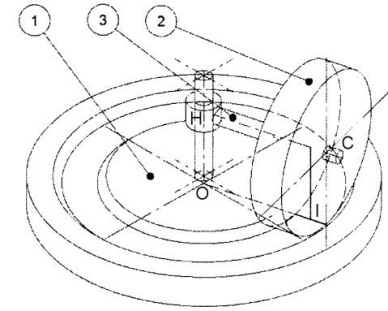
\includegraphics[width=\textwidth]{fig_06}
%\end{center}
%\end{minipage}
%
%
%
%
%\begin{minipage}[c]{.45\linewidth}
%Schéma simplifié : on considère la roue 2 comme un disque. 
%\begin{center}
%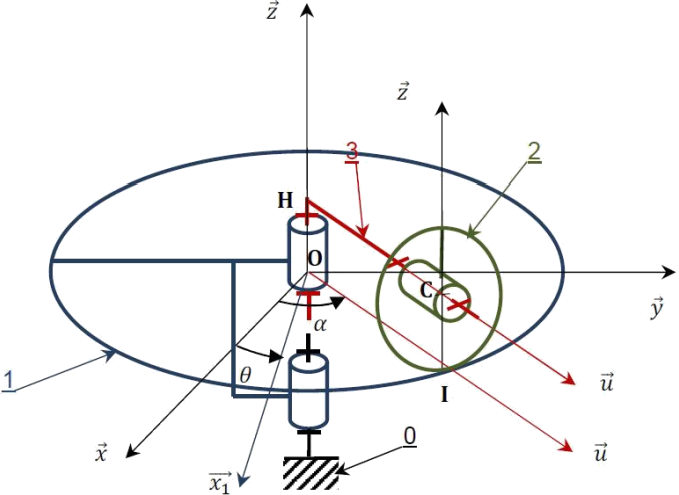
\includegraphics[width=\textwidth]{fig_07}
%\end{center}
%\end{minipage} \hfill
%\begin{minipage}[c]{.53\linewidth}
%
%Le paramétrage est le suivant : 
%\begin{itemize}
%\item $\mathcal{R}_0\left( O,\vect{x},\vect{y},\vect{z}\right)$  est associé au bâti 0 considéré comme fixe;
%\item le plateau tournant 1, de repère associé $\mathcal{R}_1\left( O,\vect{x_1},\vect{y_1},\vect{z_1}\right)$, est en mouvement de rotation d’axe $\left(O,\vect{z}\right)$ par rapport au bâti 0 tel que $\vect{z}=\vect{z_1}$ et $\theta=\left(\vect{x},\vect{x_1}\right)$;
%\item le bras 3, de repère associé $\mathcal{R}_3\left( H,\vect{u},\vect{v},\vect{w}\right)$ est en mouvement de rotation d’axe $\left(O,\vect{z}\right)$ par rapport au bâti 0 tel que $\vect{z}=\vect{w}$ et $\alpha = \left(\vect{x},\vect{u}\right)$;
%\item l’ensemble pneumatique + jante 2, de repère associé, $\mathcal{R}_2\left( O,\vect{x_2},\vect{y_2},\vect{z_2}\right)$ est en mouvement de rotation d’axe $\left(H,\vect{u}\right)$ par rapport au bras 3 tel que $\vect{u}=\vect{x_2}$ et $\beta = \left(\vect{z},\vect{z_2}\right)$. On pose $\vect{HC}=d\vect{u}$ (d est constante). Le pneumatique de rayon $r$ est en contact au point $I$ avec le plateau 1. 
%\end{itemize}
%\end{minipage}
%
%\begin{Objectif}
%Déterminer la relation entre les vitesses de rotation des 3 actionneurs permettant de reproduire 
%des conditions de roulement sans glissement d’un pneumatique sur une route. 
%\end{Objectif}
%%\subparagraph{}
%%\textit{Quelle condition le vecteur $\vectv{I}{2}{1}$ doit-il satisfaire pour assurer le maintien du contact entre 
%%les solides 2 et 1 au point I. }
%%\ifprof
%%\begin{corrige}
%%\end{corrige} \else \fi
%
%\subparagraph{}
%\textit{Quelle condition le vecteur $\vectv{I}{2}{1}$ doit-il satisfaire pour assurer le maintien du contact entre les solides 2 et 1 en $I$.}
%
%\subparagraph{}
%\textit{Déterminer $\vectv{I}{2}{1}$.}
%\ifprof
%\begin{corrige}
%\end{corrige} \else \fi
%
%\subparagraph{}
%\textit{Déterminer le vecteur vitesse de glissement au point $I$.}% selon 2 méthodes différentes.}
%\ifprof
%\begin{corrige}
%\end{corrige} \else \fi
%
%\subparagraph{}
%\textit{Dans les conditions de roulement sans glissement en $I$, en déduire la relation entre $\dot{\theta}$, $\dot{\alpha}$, $\dot{\beta}$ (vitesses de rotation des 3 actionneurs) et les dimensions du système.}
%\ifprof
%\begin{corrige}
%\end{corrige} \else \fi
%
%\subparagraph{}
%\textit{En déduire dans ce cas, l’axe instantané de rotation de 2/1.}
%\ifprof
%\begin{corrige}
%\end{corrige} \else \fi
%
%\subparagraph{}
%\textit{Préciser les composantes de roulement et de pivotement en $I$.}
%\ifprof
%\begin{corrige}
%\end{corrige} \else \fi
%
%\ifprof
%\else
%\end{multicols}
%\fi
